%!TEX root = ThesisLKN.tex

\chapter{Implementation Details} \label{chapter:4}

In this chapter, the details on implementations will be described. In detail, how the ground truth data used for training network are generated from simulated human trajectories is described in Section \ref{sec:traj_sim}. In Section \ref{sec:training}, the details on training CNNs are provided. Section \ref{sec:BOFMP_implementation} introduces the code structure of implementing BOFMP. Finally, hyperparameters in the BOFMP tracking algorithm are introduced in Section \ref{sec:hyperparameter}.

\section{Human Trajectory Simulation} \label{sec:traj_sim}

Neural networks are able to capture complex structures in data. For this reason, we train a neural network so that it can be used to extract human motion patterns from static maps. In order to make the network generalizes well, a large amount of human trajectory data in different indoor environments are needed. However, recording human trajectories with 2D laser scans in various indoor environments is expensive, since the hardwares have to be transported to different locations. Besides, since our model requires cell-specific motion patterns, the recorded human trajectories need to cover each discretized cell on the gird map. Even if it is feasible, this requires a lot of time for the laser scanner to work. To collect such a huge amount of real human trajectories is obviously out of the scope of this thesis. As a workaround, we simulated human trajectories on real-world SLAM-generated maps and those simulated trajectories are used for extracting human motion patterns. To validate our method, we evaluate our tracking algorithm on data recorded from real world. 

The maps on which human trajectories are sampled from are floor plans of indoor environments such as laboratories and offices. We assume that human motions in these environment are only constrained by the spatial configurations. Other factors, such as time, social forces and different functional areas, are not modeled. In total, we simulate human trajectories on eight maps, with a total free space area of more than \( 6.6\times10^3 \, m^2 \). Two of those eight maps are shown in Figure \ref{fig:maps}. Each pixed of the map represents a cell on its corresponding occupancy grid, and has resolution of $0.2$ $m/pixel$.

\begin{figure}[ht]
  \centering
    
\includegraphics[width=.8\textwidth, height=.3\textwidth]{figures/map1.png}
    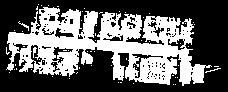
\includegraphics[width=.8\textwidth, height=.3\textwidth]{figures/map2.png}
    \caption[Two example maps on which human trajectories are sampled from.]{Two example maps on which human trajectories are sampled from. White areas are walkable, and black areas are desks or walls that human cannot walk through.}
    \label{fig:maps}
\end{figure} 

We use A* algorithm to calculate human trajectory between two points on a map. The A* algorithm is a well-know algorithm for path planning. In each iteration of its main loop, A* algorithm decides which step to take based on the summation of two values: one value represents the cost from start to current node and the other represents a heuristic estimate of cost from current node to the goal. The path found by A* algorithm replicates human trajectory, since people normally have a clear goal location in their mind (thus a heuristic estimation) and take a path that requires least efforts to reach it. To account for the fact that human tend to walk some distances away from an obstacle (e.g., people walk in the middle areas of a corridor, which are distant to walls on both sides), we apply two Gaussian filters with different widths on the static maps to get cost maps.  

The actual process from sampling trajectories to obtaining conditional probabilities as motion patterns are implemented in three steps:

\begin{my_enumerate}
\item Sampling trajectories on the full map. In order to get motion dynamics at all possible locations, we sample a predefined number of trajectories with every empty cell on the map as start location. The goal location for each trajectory is randomly sampled but the distance between start location and end location must be within a predefined range. After the start and goal location are defined, a trajectory is calculated by A* algorithm.
\item Calculate probabilities based on trajectories. A \textit{transition} is defined in this context as a person moves from cell $a$ to $c$ through $b$, i.e., $a \rightarrow b \rightarrow c$, where $a$ and $c$ are neighboring cells of $b$. If we consider eight neighboring cells, for each cell it has $8\times8=64$ different transitions. A helper function $v(c_1,c_2)$ is also defined to calculate the velocity from cell $c_1$ to $c_2$. Assume a cell $c$ is identified by its coordinates on $x$, $y$ axis, i.e, $pos(c)=(c_x, c_y)$, then
\[v(c_1, c_2)=\frac{pos(c_2)-pos(c_1)}{\Delta t}\]
Firstly a tensor $C$ is initialized to store these transition counts. So far, Tensor $C$ has 6 dimension of $32\times32\times3\times3\times3\times3$, with first two dimensions representing spatial size of a map window, next two dimensions representing $V^{en}$ and last two dimensions representing $V^{ex}$. For example, for transition $a \rightarrow b \rightarrow c$, we increment the following entry of $C$:
\[ C(pos(b), v(a, b), v(b, c))\]
For each sampled trajectory, we add every transition along this trajectory to its corresponding entry in $C$. The conditional probability $P_i(V^{ex}|V^{en})$ is then calculated from transition counts tensor $C$ as:
\begin{equation}
P_i(V^{ex}=v_1|V^{en}=v_0) = \frac{C(pos(i), v_0, v_1)}{\sum_{ v}C(pos(i), v_0, v)}
\end{equation}
\item Sampling map window with fixed size and data augmentation. The map window that we feed into our network is of size $32\times32$ cells (i.e., $6.4 \times 6.4$m). Therefore, we randomly crop a predefined number of map windows from the whole map. If a map window has free space less than $50\%$, it is not used. To increase the number of data samples, each map window is augmented eight times: for both the map window and its horizontal mirroring, they are rotated by $90^\circ$, $180^\circ$ and $270^\circ$. 

  So far, the ground truth of each map window has same dimensions as $C$, i.e, $32\times32\times3\times3\times3\times3$. However, since the output of network has at most three dimensions, the ground truth has to be resized to $32\times32\times64$, without considering velocity $v=(0, 0)$.
\end{my_enumerate}

The above algorithm is described in Algorithm \ref{algo:data_generation}. 

\begin{algorithm}
\caption{Algorithm for generating data for neural network.}
\label{algo:data_generation}
\begin{algorithmic}[1]
\Procedure{SamplingTrajectories(map, n)}{}
\State $allTrajectories \gets \emptyset$
\For{\textit{cell} in \textit{emptyCells(map)}} 
    \Comment loop over all empty cells on map
	\State $trajectories \gets \emptyset $
	\State $tries \gets 0$
	\While{$tries < N $} 
	\Comment try to sample $N$ trajectories for each cell
	\State $start \gets cell$
	\State $goal \gets sampleGoalLocation(map, start)$
	\State $trajectory \gets AStar(start, goal)$
	\If {$isValid(trajectory)$} 
		\Comment check whether $trajectory$ is empty
		\State \textbf{add} $trajectory$ \textbf{to} $trajectories$
	\EndIf
	\State $tries \gets tries+1$
	\EndWhile
	\State \textbf{append} $trajectories$ \textbf{to} $allTrajectories$
\EndFor
\State \Return $allTrajectories$
\EndProcedure
\\
\Procedure{GetConditionalProbs(Trajectories)}{}
\State Initialize $C$ with zeros
\For{\textit{trajectory} $(c_1, \cdots, c_n)$ in \textit{trajectories}} 
    \Comment loop over all sampled trajectories
    \For{$t=2:n-1$}
    \Comment add transition $c_{t-1} \rightarrow c_t \rightarrow c_{t+1}$
	\State  $idx \gets (pos(c_t), v(c_{t-1}, c_t), v(c_t, c_{t+1}))$
	\State $C(idx) \gets C(idx)+1$ 
    \EndFor
\EndFor
\State $probs \gets calculateProbs(C)$
\State \Return $probs$
\EndProcedure
\\
\Procedure{CropMapWindow(map, probs, S)}{}
\State $data \gets \emptyset$ 
\State $count \gets 0$
\While{$count < S$}
	\Comment try to get $S$ samples
    \State $loc \gets sampleRandomLocation(map)$
    \State $window \gets getWindow(map, loc)$
    \If {$freeSpace(window) < 0.5$}
    	\State \textbf{continue}
    \EndIf
    \State $probWindow \gets getProbWindow(probs, window)$
    \State \textbf{add} $(window, probWindow)$ \textbf{to} $data$
    \State \textbf{add} $agument(window, probWindow)$ \textbf{to} $data$
    \State $count \gets count+1$
\EndWhile

\State \Return $data$
\EndProcedure
\end{algorithmic}
\end{algorithm}

\section{Architecture of Neural Network} \label{sec:training}

As described in Section \ref{sec:cnn}, our network architecture is similar to that of \citet{jegou2017one}, with a minor difference in the last layer (i.e., the output layer). For their use in semantic classification, the input $\mathbf{v}$ to the last year has dimensions of $W\times H \times N$. The first two dimensions are spatial size of the input image, and last dimension corresponds to number of semantic classes. The last layer, known as spatial softmax layer, applies the following function.
\[\varphi(\mathbf{v})_{x, y, j} = \frac{e^{\mathbf{v}_{x, y, j}}}{\sum_{n=1}^N e^{\mathbf{v}_{x, y, n}}}\]
In other words, the output of last layer are class scores that can be interpreted as probabilities. In our case, since the network has to output conditional probabilities $P_c({V^{ex}|V^{en}})$ for all possible $V^{en}$, there are essentially eight probability distributions existing in $\mathbf{v}$. Therefore, our last layer has to firstly segment values to its corresponding $V^{en}$, then apply softmax accordingly. 

\begin{figure}[H]
  \centering
    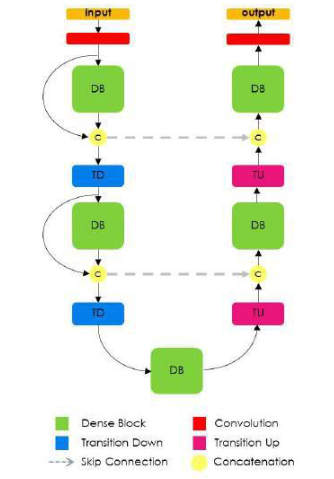
\includegraphics[width=.45\textwidth]{figures/tiramisu.png}
    \caption[Illustration of the fully convolution DenseNet.]{Illustration of the fully convolution DenseNet in \citep{jegou2017one}. The network consists of a downsampling path extracting high-level semantic features and an upsampling path recovering outputs to full resolution as input image. The skip connections, as indicated by dashed lines, combines both deep coarse features and shallow fine features.}
    \label{fig:tiramisu}
\end{figure}

The overall architecture of the network is depicted in Figure \ref{fig:tiramisu}, and how each component is structured is summarized in Table \ref{table:components}. For the network that we use in this thesis, it has 31 convolutional layers, 13 in the downsampling path, 5 in the bottleneck dense block, and 13 in the upsampling path. Two max pooling layers are used to downsample the spatial size of inputs, and two deconvolution layers are used to recover outputs' resolution. Each dense block consists of 5 layers. One important parameter for dense block is the \textit{growth rate}, which is the number of feature maps in each layer. We use a growth rate of 12. Thus, the output of each dense block has $5 \times 12 = 60$ feature maps. The number of feature maps at the end of blocks is listed in Table \ref{table:number_feature_maps}. The network has in total 448,648 parameters.

\begin{table}[H]
\centering  
\begin{tabularx}{.9\textwidth}{c|c}
    \hline
    Component            & Structure            \\ \hline \hline
    Transition Down (TD) & BN $\rightarrow$ RELU $\rightarrow$ $1 \times 1$ CONV $\rightarrow$ $2 \times 2$ MAXPOOL \\ \hline
    Transition Up (TU)   & $3 \times 3$ DECONV with stride 2 \\
   \hline
   Layer                 & BN $\rightarrow$ RELU $\rightarrow$ $3 \times 3$ CONV \\ \hline
   Dense Block (DB).     & 5 Layers that are densely connected \\ \hline
  \end{tabularx}
\caption{Structure of each component in Figure \ref{fig:tiramisu}.}
\label{table:components}
\end{table}

\begin{table}[H]
\centering  
\begin{tabularx}{.53\textwidth}{c|c}
    \hline
    Blocks            & Number of feature maps            \\ \hline \hline
    Input                &    1 \\ \hline
    CONV + DB + C        &    68 \\ \hline
    TD + DB + C          &    128 \\ \hline
    TD                   &    128 \\ \hline
    DB + TU + C          &    188 \\ \hline
    DB + TU + C          &    128 \\ \hline
    DB + CONV            &    64 \\ \hline
    Softmax           &    64 \\ \hline
  \end{tabularx}
\caption{Number of feature maps at the end of blocks.}
\label{table:number_feature_maps}
\end{table}

\newpage
\section{Preprocessing of Tracking Data}

To evaluate our method, we apply the BOFMP filter on real data that are recorded by laser scanners. The real data records occupancy information on a static map which changes over time. Since occupancy indicates a person's location on the map, the time-varying occupancy is able to represent human trajectories. We define the real data that records occupancy information on a given map window for a certain amount of time as a \textbf{scene}. After preprocessing, each scene records human trajectories on that map window so that we can evaluate our method on. However, due to various reasons, such as localization error of robots and discretization errors, the real data could be very noisy. Therefore, a preprocessing pipeline is proposed. It consists of following steps:

\begin{my_enumerate}
\item \textbf{Downsample}. The real data are recorded by laser scanners with frequency of 12Hz, which means we get 12 frames of data per second. Human walking speed in office is roughly 1$\sim$1.2 $m/s$. Since the map resolution is 0.2 $m$, this means for moving one cell in map it takes roughly 2$\sim$2.4 frames. Therefore, We decide to downsample real data by merging the occupancy in 3 continuous frames to 1 frame.
\item \textbf{Remove static occupancy}. A scene is supposed to show the \textit{dynamic} changes of occupancy which represent human trajectory. Therefore, if a cell is occupied over a quarter of the time in a scene, it is likely to be sensor failure and therefore should be removed. 
\item \textbf{Remove occupancies near walls}. According to our observations on the recorded data, it is very likely that the occupied cells near walls are false positive due to discretization errors. Therefore, we remove occupancies that are one cell away from walls. 
\item \textbf{Remove outliers.} A person in the real data are represented as a blob of occupied cells. Therefore, if there is a single occupied cell, it is thought to be sensor noise and thus should be removed.
\end{my_enumerate}

Figure \ref{fig:preprocessing} shows a scene at certain time steps. The upper plot shows the original data before preprocessing and the lower shows after preprocessing. One can see that, after preprocessing, the noisy occupancies are removed without affecting the dynamics of human motion.

Even after preprocessing, we found there are still a lot of scenes which do not show proper occupancy information. For example, there might be no occupied cells for a long period of time. On the other hand, classification on trajectories with different motions (e.g., going straight or making a turn) might be interesting for future work. Therefore, we developed a small application to filter out useless scenes and classify scenes into a set of predefined motion classes based on the underlying trajectory. A screenshot of the application is shown in Figure \ref{fig:application}.

\begin{figure}[ht]
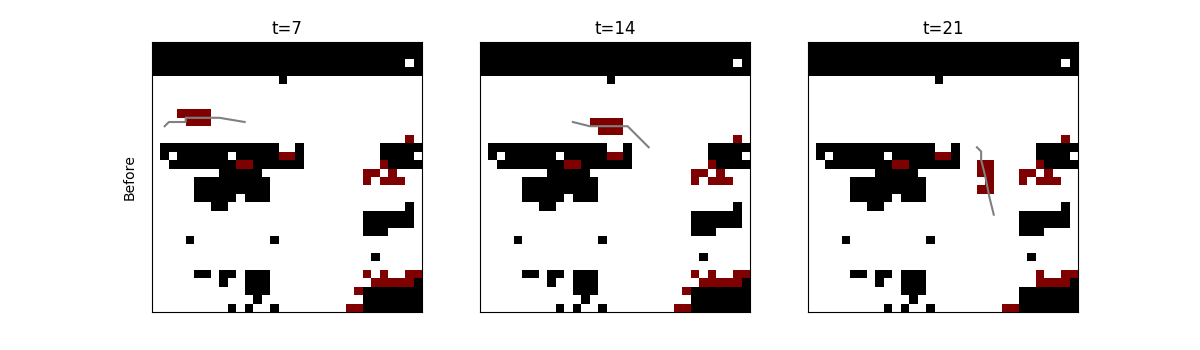
\includegraphics[width=\textwidth]{figures/before.png} \\
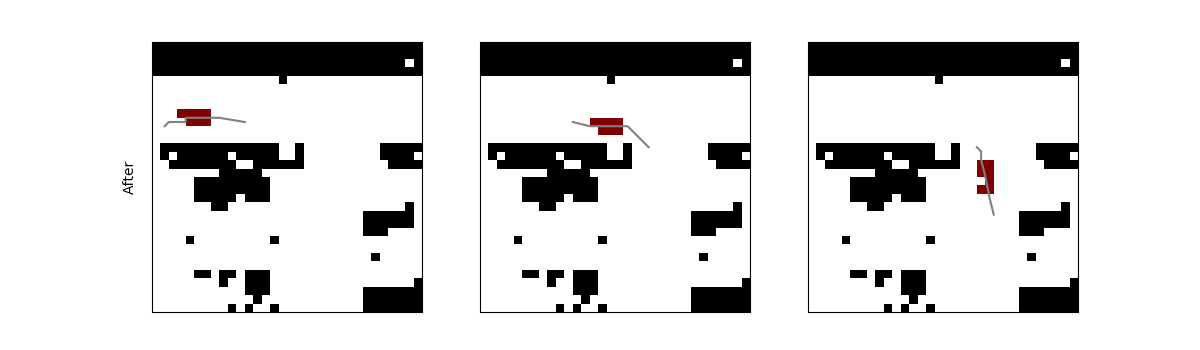
\includegraphics[width=\textwidth]{figures/after.png}
\caption[One example of preprocessing of real data.]{One example of preprocessing of real data. Black cells are from the static map. Red and white cells represent \textit{occupied} and \textit{not occupied} respectively. A person is identified by a blob of occupied cells and the gray line indicates the trajectory. \textbf{Upper}: The real data recorded by laser scanners. \textbf{Lower}: The corresponding data after preprocessing. One can see that, the noisy occupancies are removed without affecting the dynamics of human motion.} 
\label{fig:preprocessing}
\end{figure}

 \begin{figure}[H]
\centering
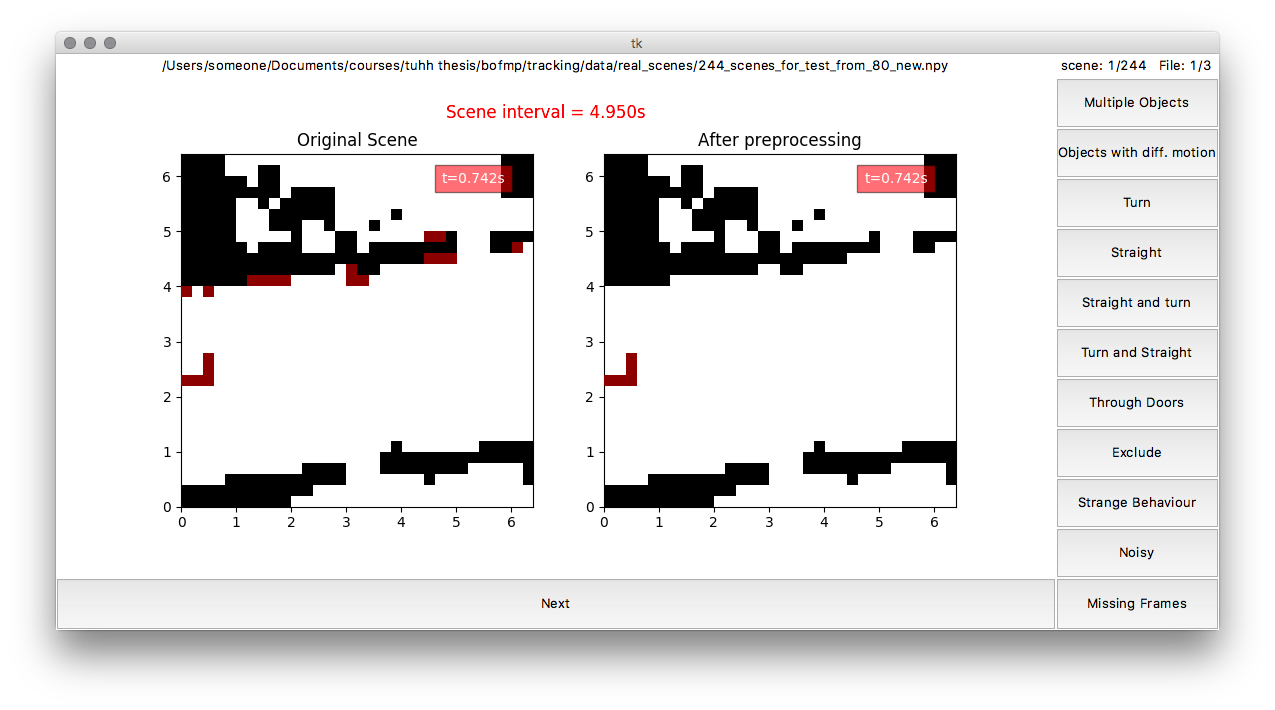
\includegraphics[width=.9\textwidth]{figures/application_1.png}
\caption[Application used for labeling scenes.]{Application used for labeling scenes. User can define their own classes, which are shown as buttons on the right. On the left, both the original scene and preprocessed scene are displayed as animations. User can continue labeling by clicking ``Next'' button.} 
\label{fig:application}
\end{figure}

\section{Implementation of BOFMP} \label{sec:BOFMP_implementation}

\subsection{Extension of Network Output} \label{sec:mm_ext}

As described in Section \ref{sec:traj_sim}, the motion pattern extracted from network output considers max speed of 1 $cell/timestep$. However, since human does not always walk in a constant speed, we need to adapt our motion model to higher speeds. This is done by applying Gaussian blur in acceleration space. For now, we omit the cell index $c$, and the motion pattern from network output is represented as:
\begin{equation}
P_{NN}(v^{ex}=(v^{ex}_x, v^{ex}_y)|v^{en}=(v^{en}_x, v^{en}_y)) \label{eq:mm_1}
\end{equation}

where $v^{ex}_x, v^{ex}_y,v^{en}_x, v^{en}_y \in [-1, 1] \cap \mathbb{Z}$. We define the \textit{extent} as the number of values that velocity can take in either $x$ or $y$ axis. Due to its symmetry, the max speed for extent $e$ is $\lfloor \frac{e}{2} \rfloor$ cell/step. Therefore, $P_{NN}$ has an extent $e_{n}$ of 3 and dimension of $3 \times 3 \times 3 \times 3$. 

Let us assume that we want motion model for extent $e_w$. This is achieved by firstly padding $P_{NN}$ to dimension $e_w \times e_w \times e_w \times e_w$ with zeros, s.t., $v^{ex}_x, v^{ex}_y,v^{en}_x, v^{en}_y \in [-\lfloor \frac{e_w}{2} \rfloor, \lfloor \frac{e_w}{2} \rfloor] \cap \mathbb{Z}$ . Then we can calculate the probabilities for acceleration conditioned on entering velocity:
\begin{equation}
P_{NN}(a|v^{en}) = P_{NN}(v^{ex}=v^{en}+a|v^{en}) \label{eq:mm_2}
\end{equation}

With a 4-dimensional Gaussian kernel $K(a, b) \sim \mathcal{N}((a,b), \Sigma)$, we have:
\begin{equation}
P(a|v^{en}) = \sum_{\hat{a}, \hat{v}^{en}}P_{NN}(\hat{a}|\hat{v}^{en})\times K(\hat{a}, \hat{v}^{en}) \label{eq:mm_3} 
\end{equation}

Finally we get motion pattern $P(v^{ex}|v^{en})$ by restoring to velocity space and normalization:
\begin{align}
\hat{P}(v^{ex}|v^{en}) &= P(a=v^{ex}-v^{en}|v^{en}) \\
P(v^{ex}|v^{en}) &= \frac{\hat{P}(v^{ex}|v^{en})}{\sum_{v^{ex}}\hat{P}(v^{ex}|v^{en})} \label{eq:mm_4}
\end{align}

One example is shown in Figure \ref{fig:mm_ext}. As can be seen from the figure, the original motion pattern $P_{NN}(v^{ex}|v^{en}$ has max speed of 1 $cell/step$, while for the extend one $P(v^{ex}|v^{en})$ the max speed is 2 $cell/step$. From the extended motion pattern $P(v^{ex}|v^{en})$, one can see that only the directions of velocity change but not the speed. This implies that even if a person changes his or her walking direction, the walking speed is normally not changed.

\begin{figure}[hp]
\begin{tabular}{cc}
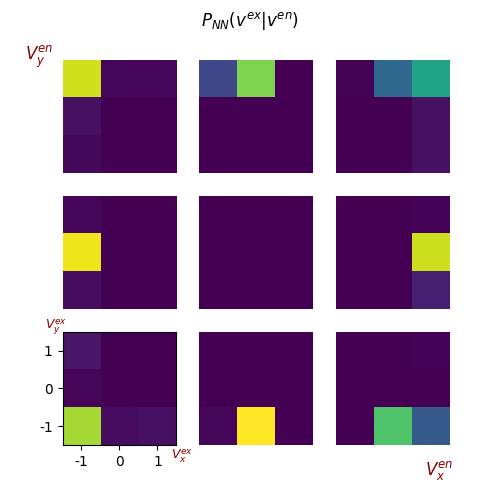
\includegraphics[width=0.5\textwidth]{figures/mm_ext_1.png}
&
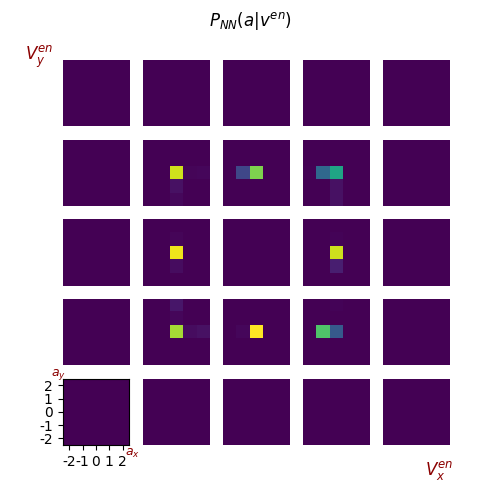
\includegraphics[width=0.5\textwidth]{figures/mm_ext_2.png} \\
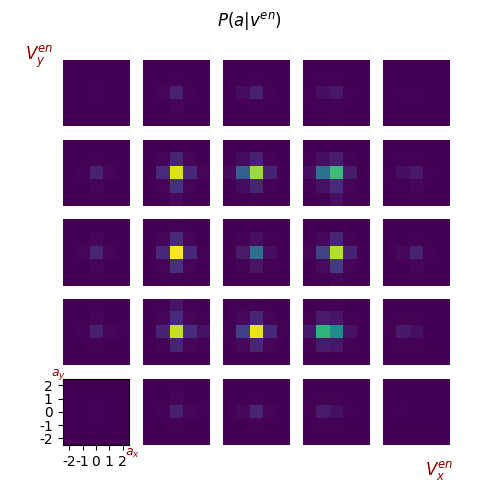
\includegraphics[width=0.5\textwidth]{figures/mm_ext_3.png}
&
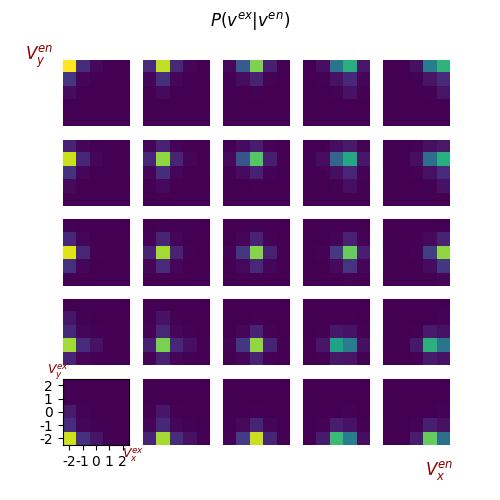
\includegraphics[width=0.5\textwidth]{figures/mm_ext_4.png}
\end{tabular} 
\caption[One example of extending motion pattern probabilities from network output to higher extent.]{One example of extending motion pattern from network output to higher extent. The definitions of these quantities shown in figure are explained in Equation \ref{eq:mm_1} $\sim$ \ref{eq:mm_4}. The original motion pattern $P_{NN}(v^{ex}|v^{en})$ has max speed of 1 $cell/step$, while for the extend one $P(v^{ex}|v^{en})$ the max speed is 2 $cell/step$. This is achieved by applying Gaussian blurring in acceleration space. From the extended motion pattern $P(v^{ex}|v^{en})$, one can see that only the directions of velocity change but not the speed (in fact, with a small probability to accelerate or decelerate). This implies that even if a person changes his or her walking direction, the walking speed is normally not changed.} 
\label{fig:mm_ext}
\end{figure}

\subsection{Workflow of BOFMP}

Before introducing the workflow of our method, some parameters that used to initialize BOFMP must be clarified:

\begin{my_enumerate}
\item \textbf{extent \( e\)}. As introduce in \ref{sec:mm_ext}, extent is defined as the number of values that velocity can take in either $x$ or $y$ axis.	For example, if extent is 7, the velocities on both $x$ and $y$ axis must be integers within range  \( [-3, 3] \). The extent determines the maximum speed speed our algorithm concerns. 
\item \textbf{variance \( \delta^2\)}. For BOFUM, this parameter refers to the variance of the Gaussian distributed acceleration noise in Equation \ref{eq:adding_noise}. For BOFMP, it is the variance of the Gaussian kernel used for blurring in Equation \ref{eq:mm_3}. In both cases, this parameter reflects the algorithm's belief on how likely an object accelerates or decelerate.
\item \textbf{omega \( \Omega \)}. In the correction step of BOF filters, measurements from sensors are taken into account for estimating the posterior probability. Since sensor could be noisy, this parameter determines how much does the filter trusts the measurements. The sensor used for in our tracking application is laser scanners, which is rather physically reliable and therefore has a low \( \Omega \) value.
\end{my_enumerate}

A trained CNN model that used for extracting motion pattern from static map must be available. With the above parameters being defined and the CNN model being ready, the BOFMP filter can be applied. Firstly, feed the static map to the network so that $P_{NN}(V^{ex}|V^{en})$ is retrieved. It is then extended to the desired extent $e$ to get motion pattern $P(V^{ex}|V^{en})$. Before the filtering starts, the occupancy and velocity probabilities are initialized uniformly, i.e. for $c=1:N$,
\begin{gather}
P(O_c = occ) = P(O_c = nocc)=0.5 \\
P(V_c=v) = \frac{1}{e^2}
\end{gather}

 After initialization, the actual tracking can start by recursively executing tracking step. A tracking step is composed of two steps: \textit{prediction} and \textit{estimation}. In prediction step, a prior distribution of the state of cells is derived. In estimation step, a posterior distribution is calculated by multiplying the prior distribution with a conditional probability distribution that represents correction based on incoming measurements. However, the measurement gives information about only whether a cell is occupied or not at each time step. In order to make proper predictions for the next time step, the filter has to infer velocities for each cell. To get some intuitions, Figure \ref{fig:correction} shows an example of tracking step. The complete workflow is illustrated in Figure \ref{fig:fitering_workflow}.

\begin{figure}[H]
  \centering
    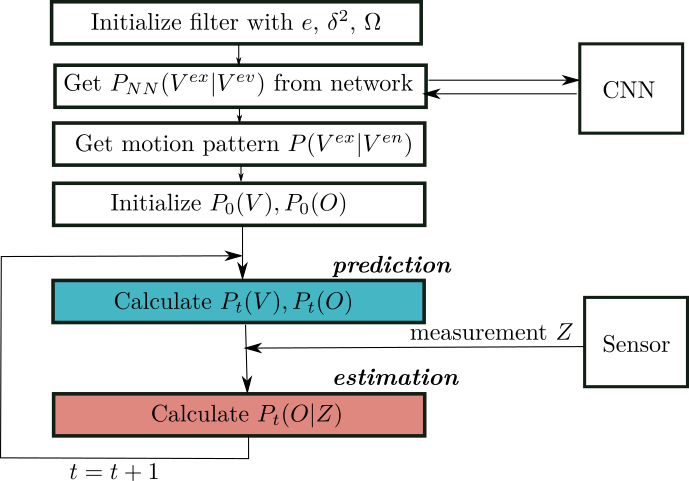
\includegraphics[width=.7\textwidth]{figures/filtering_workflow.png}
    \caption[Workflow of BOFMP filter.]{Workflow of BOFMP filter. The parameters of the filter have to be defined firstly. The motion pattern probabilities are obtained from the outputs of a pre-trained CNN. The state of cells are initialized with uniform distributions and then recursively updated by prediction and estimation step. Measurements from sensor are used for estimation.}
    \label{fig:fitering_workflow}
\end{figure}

\begin{figure}[ht]
  \centering
    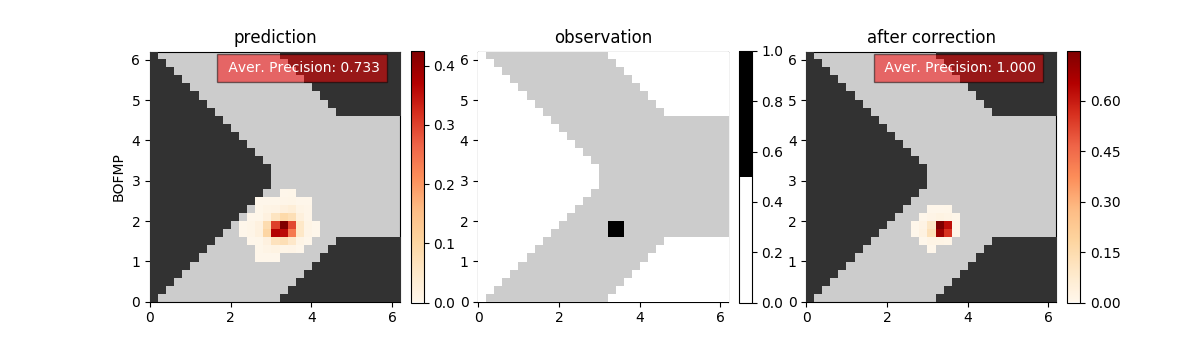
\includegraphics[width=\textwidth]{figures/correction_step.png}
    \caption[One filtering step of BOFMP filter.]{One filtering step of BOFMP filter. At last time step, the person goes from up to down. Based on motion pattern, BOFMP predicts that there are possibilities that this person will turn to left-down and keep going downwards. After measurement shows that this person still goes downwards, BOFMP corrects its predictions and attenuates probabilities of turning left-down. Since the measurement adds additional information for BOFMP to make better predictions, the average precision increases after correction step.}
    \label{fig:correction}
\end{figure}

\subsection{Code Structure}

The functionalities of the code concern mainly three parts:
\begin{my_enumerate}
\item \textbf{Tracking filters}. Both BOFMP and the baseline BOFUM filters are implemented. Besides, based on the data used, i.e., either simulated data or real data, the implementation has to be different. 
\item \textbf{Visualization of tracking}. To have a better idea about how tracking performs, visualization of tracking for each time step is necessary. We implemented two ways of visualization. One is to show tracking step by step as prediction and correction with static plots. The other shows the tracking process with animation. 
\item \textbf{Evaluation on tracking performance}. In order to compare our method with its baseline, evaluation on tracking performance is necessary. The metric used for evaluation is described in Section \ref{sec:metrics}.
\end{my_enumerate}

We follow an object-oriented programming paradigm. By defining classes and subclasses, this facilitates code reuse and better structure of the code. Figure \ref{fig:classes} shows the main classes defined in the code. They are grouped based on their functionalities. 

\begin{figure}[hp]
  \centering
    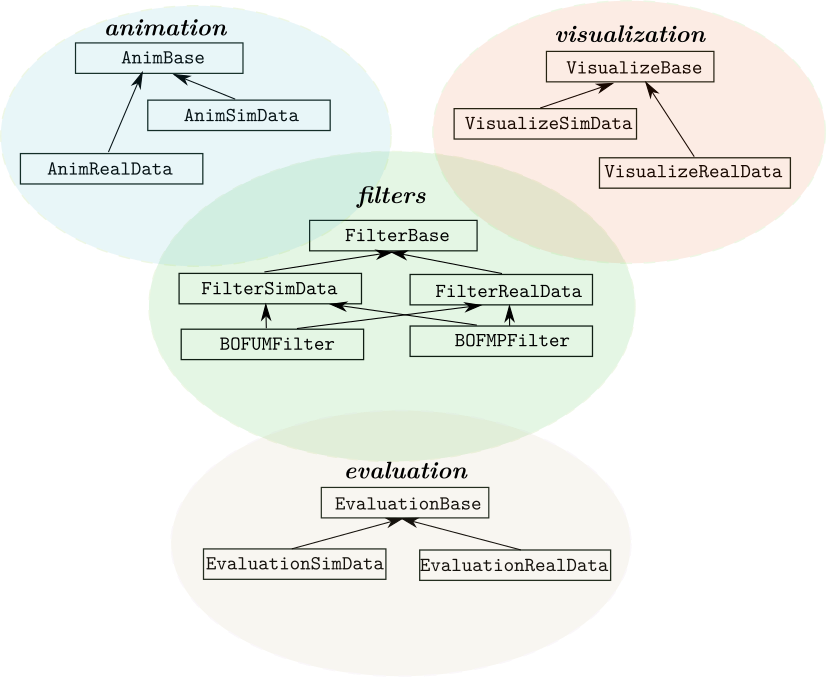
\includegraphics[width=\textwidth]{figures/classes.png}
    \caption[Classes defined in the code.]{Classes defined in the code. Classes are grouped according to their functionalities. The ``filters'' is shown in the center since it is used by other classes. The arrows show class inheritance. For example, \texttt{ClassA} $\rightarrow$ \texttt{ClassB} indicates that \texttt{ClassA} is inherited from \texttt{ClassB}. }
    \label{fig:classes}
\end{figure}

